%%%%%%%%%%%%%%%%%%%%%%%%%%%%%%%%%%%%%%%%%%%%%%%%%%%%%%%%%%%%%%%%%%%%%
%
% Enonce de projet, Cotonou Juillet 2021
%
%%%%%%%%%%%%%%%%%%%%%%%%%%%%%%%%%%%%%%%%%%%%%%%%%%%%%%%%%%%%%%%%%%%%%

\documentclass[12pt]{article}
\usepackage[utf8]{inputenc}
\usepackage{amsmath}
\usepackage{amsfonts}
\usepackage{amssymb}
\usepackage{graphicx}
\graphicspath{{figures/}}
%\usepackage{beamerthemesplit}
%\usepackage{beamerthemeshadow} 
\usepackage{color}
\usepackage{hyperref}
\usepackage{xspace}
\usepackage{xifthen}
\usepackage{multicol}
\usepackage{mathtools}
\usepackage{algorithm,algorithmic}
\usepackage{dsfont}
%
% these 2 next needed for mathbb greek letters
\usepackage{breqn} 
\usepackage[bbgreekl]{mathbbol}
%
\usepackage{bbm} % this one is needed for the indicator
%

% custom commands in sty file, for easier writting and change of notations
\usepackage{my_notations}

\title{Enoncé du projet pour le cours d'optimisation}
\date{Juillet 2021 \\
Ecole d'Eté en Intelligence Artificielle \\
fondation Vallet\\
Cotonou, Bénin}
\author{}

%%%%%%%%%%%%%%%%%%%%%%%%%%%%%%%%%%%%%%%%%%%%%%%%%%%%%%%%%%%%%%%%%%%%%
\begin{document}
\maketitle

\section{Prise en main du code, intuition sur les fonctions}
Aller dans le répertoire \texttt{Project}. 
\begin{enumerate}

\item Ouvrir \texttt{3Dplots}. C'est un fichier pour dessiner des fonctions en \texttt{d<-2} dimensions (``contour plots'' et ``plot 3D''). 
Dessiner plusieurs des fonctions données dans \texttt{test\_functions}\footnote{Les fonctions de \texttt{test\_functions} marchent avec des dimensions arbitraires}.
Il suffit de changer le champ \texttt{fun<-} et mettre le nom de la fonction à dessiner
(par exemple \texttt{fun<-quadratic} ou \texttt{fun<-rosen} ou \texttt{fun<-ackley}, \ldots). \\
\begin{enumerate}
\item Repérer quelles fonctions sont multimodales (i.e., ont plusieurs optima locaux différents).
\item Changer la position de l'optimum \texttt{glob\_xstar} et le conditionnement \texttt{cond.no} de la fonction \texttt{quadratic}. Regarder l'effet sur les dessins. La fonction \texttt{quadratic} est une fonction test fondamentale pour le développement théorique et pratique des optimiseurs: 
c'est la fonction la plus simple qui possède un minimum, et on peut considérer que localement autour des optima locaux toutes les fonctions sont quadratiques (d'après le développement de Taylor à l'ordre 2).
\end{enumerate}

\item Ouvrir \texttt{mainOptim}. Il s'agit du programme principal qui permet de 
\begin{itemize}
\item formuler le problème (liste \texttt{PbFormulation}): choisir une fonction (champ \texttt{fun}), son nombre de dimensions (champ \texttt{d}), ses bornes (champs \texttt{LB,UB})
\item choisir les paramètres de l'algorithme d'optimisation (liste \texttt{optAlgoParam}).
Ici ce sont les paramètres des variantes de la méthode de descente vues en cours: des critères d'arrêt (champs \texttt{budget}, \texttt{minGradNorm}, \texttt{minStepSize} ), l'activation de la recherche en ligne (\texttt{linesearch\_type <- "armijo"}) ou non (\texttt{linesearch\_type <- "none"}), la méthode d'estimation de la direction de recherche (\texttt{direction\_type <- "gradient"} ou \texttt{"momentum"} ou \texttt{"NAG"}), le facteur de taille de pas quand la recherche en ligne n'est pas active (\texttt{stepFactor}), le coefficient de mémoire \texttt{beta} des accélérations de gradient, \ldots
\end{itemize}
\begin{enumerate}
\item Avec la fonction \texttt{quadratic} et un point initial pas trop proche de l'optimum \texttt{glob\_xstar}, observer l'effet de \texttt{stepFactor} sur les itérations quand il n'y a pas de recherche en ligne (\texttt{linesearch\_type <- "none"}). Remarquer qu'en partant du même point avec la recherche en ligne (\texttt{linesearch\_type <- "armijo"}), la convergence a lieu, au prix de quelques évaluations supplémentaires à chaque itération.
\item  La fonction Rastrigin est multimodale. Sur la fonction \texttt{"rastrigin"} en \texttt{d<-2} dimensions, observer des convergences locales, i.e., des points de convergence qui sont des optima locaux mais pas globaux. Pour être sûr de bien observer le phénomène, il faut laisser l'optimiseur converger suffisamment longtemps, typiquement \texttt{budget<-10000} et le critère d'arrêt est autre que le budget.
\end{enumerate}

\end{enumerate}

\section{Etude d'une fonction de type apprentissage supervisé}
On se propose de créer une nouvelle fonction qui a un rapport étroit avec des applications en machine learning:
\begin{equation}
f(x) ~=~ \sum_{i=1}^d (x_i-c_i)^2 + \lambda \sum_{i=1}^d \lvert x_i \rvert \quad,\quad \lambda \ge 0
\label{eq:sphereL1}
\end{equation}
Le premier terme correspond à une parabole sphérique centrée en $c$ (fonction \texttt{sphere}). 
Le second terme est la norme L1 (\texttt{L1norm}) multipliée par le coefficient $\lambda$.\\
Analogie avec le machine learning: $x$ sont les poids du réseau; 
la fonction sphère est un modèle (simpliste) de l'erreur quadratique moyenne d'un réseau de neurones, erreur qui serait minimisée en $c$; 
Pour fixer les idées, faisons l'hypothèse que $c_i = i~,~i=1,\ldots,d$, ainsi les $c_i$ ont des valeurs différentes (accessoirement croissantes).
$\lambda \lVert x \rVert_1$ est le terme de régularisation, qui aide à avoir une bonne capacité de généralisation du réseau. 
Nous nous proposons d'explorer pourquoi.
\begin{enumerate}
\setcounter{enumi}{2}
\item Programmer la fonction de l'équation~(\ref{eq:sphereL1}) à la façon des autres fonctions du fichier \texttt{test_functions}.
\item La minimiser en dimension $d<-10$ avec, par défaut, la descente \texttt{"momentum"} complétée par la recherche en ligne \texttt{"armijo"}. 
Essayez plusieurs valeurs de $\lambda \ge 0$.
Que remarquez vous sur les $x^\star$ proposés? En quoi cela peut il expliquer une meilleure capacité de généralisation du réseau de neurones?
\end{enumerate}


\section{Rendre une méthode de descente un peu plus globale: redémarrages}
Nous avons vu en cours et avec la question 4.(b) que les méthodes de descentes convergent localement, ce qui peut être
un inconvénient dans les problèmes où il y a plusieurs solutions.\\
Une façon simple de remédier partiellement à ce problème est de redémarrer des descentes depuis des points différents.
\begin{enumerate}
\setcounter{enumi}{4}
\item Proposer un algorithme et le programmer qui réalise des redémarrages aléatoires de d'optimisation par descente.
\end{enumerate}

\section{Régularisation vs. nombre de points de données pour un réseau de neurones}
Reprendre le code donné dans le fichier \texttt{main\_neural\_net}: il s'agit d'un réseau de neurone utilisé 
en régression pour apprendre une fonction à 2 dimensions (donc il y a 2 entrées dans le réseau).
On se propose d'étudier le rapport entre le nombre de données d'apprentissage, \texttt{ntrain}, 
et le bon choix du paramètre de régularisation $\lambda$ (\texttt{lambda} dans le code). 
\begin{enumerate}
\setcounter{enumi}{5}
\item Essayer les valeurs : \texttt{ntrain}=5, 10 et 50, et toutes leurs combinaisons avec $\lambda=0.01,~0.1$ et 1.
Que remarquez vous sur l'erreur de test (\texttt{rmsetest}) ? Comment l'expliquez vous ? 
Que peut on dire sur l'évolution de l'erreur d'apprentissage (\texttt{rmsetrain}) dans cette campagne d'essais?
Que remarque-t-on sur les caractéristiques de solutions $x^\star$?
\end{enumerate}

\appendix
\newpage
\section{Réponses et commentaires supplémentaires}

\noindent 1.(a).\\ 
Unimodales: \texttt{sphere,quadratic,rosen,L1norm,tunnel}. AN: \texttt{sphere,quadratic,L1norm} sont convexes, pas les autres. \texttt{L1norm} est non différentiable.\\
Multimodales: \texttt{ackley,rastrigin,schwefel,michalewicz,quad\_wave}

\vskip\baselineskip
\noindent 1.(b).\\ 
Quand on augmente le conditionnement, la fonction \texttt{quadratic} ressemble de plus en plus à une vallée profonde, néanmoins rectiligne, contrairement à \texttt{rosen}.

\vskip\baselineskip
\noindent 2.(a). Le conditionnement de la fonction quadratique a un role, plus il est grand, plus \texttt{stepFactor} doit être petit. 
Si \texttt{stepFactor} est trop grand, la méthode diverge, en d'autres termes elle sort des bornes de $\mathcal{S}$. 
Vice versa, un petit \texttt{stepFactor} permet la convergence, mais à une vitesse inférieure (petits pas).
Exemple de valeurs: \texttt{xinit<-c(-4.9,-4.9)}, \texttt{cond.no<-3}, \texttt{stepFactor <- 0.01,0.1,0.9}.\\ 

\vskip\baselineskip
\noindent 2.(b). Pour trouver plus facilement des points initiaux menant à une convergence locale, générer le point initial au hasard avec
\texttt{optAlgoParam{\$}xinit <- runif(n = d,min = pbFormulation{\$}LB,max = pbFormulation{\$}UB)}

\vskip\baselineskip
\noindent 3.
\begin{center}
\begin{minipage}[b]{0.6\textwidth}
\texttt{
sphereL1 <- function(xx)\{ \\
\mbox{\quad}   lambda<-5 \\
\mbox{\quad}  y<-sphere(xx)+lambda*L1norm(xx) \\
\mbox{\quad}  return(y) \\
\}
} % end texttt
\end{minipage}
\end{center}

\vskip\baselineskip
\noindent 4. Plus $\lambda$ est grand, plus $x^\star$ s'éloigne de $c$ et tend vers 0 mais d'une façon non rectiligne: certaines composantes 
de $x^\star$, en l'occurence celles associées aux composantes basses de $c$, sont mises à 0.\\
Ceci peut être compris en remarquant le lien entre le problème~(\ref{eq:sphereL1}) et l'optimisation avec contraintes.
Le problème 
\begin{equation*}
\left\{
\begin{array}{l}
\min_x f(x) = \lVert x - c \rVert^2 \\
\text{tel que }~~ g(x) = \lVert x \rVert_1 - \tau \le 0 \quad,\quad \tau>0
\end{array}
\right.
\end{equation*}
a pour Lagrangien à minimiser sur $x$
\begin{equation*}
\min_x f(x) + \lambda^\star g(x) = \lVert x - c \rVert^2 + \lambda^\star \lVert x \rVert_1 - \lambda^\star\tau
\end{equation*}
Le dernier terme ne dépend pas de $x$, et les deux précédents sont précisément la fonction régularisée~(\ref{eq:sphereL1}).
Le dessin ci-dessous représente la fonction sphère et la limite de la contrainte sur $\lVert x \rVert_1$. On voit que la solution tend à 
se trouver sur un sommet du domaine faisable. Or, en ces sommets, des composantes de $x$ s'annulent. Notons que ce phénomène se produit de plus 
en plus quand on monte en dimensions et est moins frappant quand $d=2$.
\begin{center}
 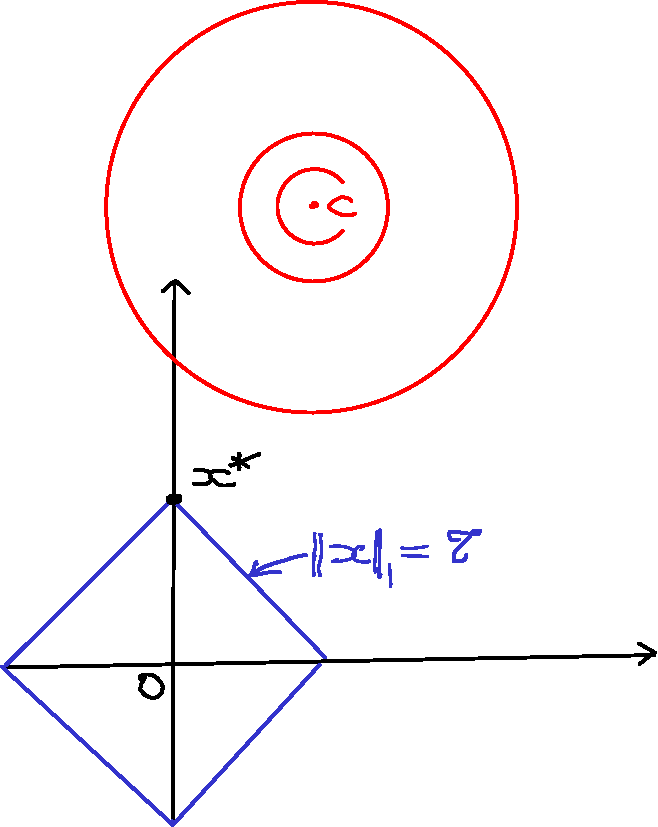
\includegraphics[width=0.5\textwidth]{l1sphere_regularization-crop.pdf}
\end{center}
Analogie machine learning: si les composantes de $x$ sont des poids de réseau de neurone, cela veut dire que certains liens dans le réseau de neurone sont supprimés.
Ainsi le réseau a une plus faible capacité à surapprendre les données, il généralise mieux. Tout l'art est de trouver la bonne valeur de $\lambda$.

\vskip\baselineskip
\noindent 5. 
\begin{center}
\begin{minipage}[t]{\textwidth}
\begin{algorithmic}
\REQUIRE \texttt{budget}, \texttt{nb\_restarts}
\FOR {\texttt{i in 1} \TO \texttt{nb\_restarts} }
\STATE \texttt{xinit <- runif(n=d,min=LB,max=UB)}
\STATE \texttt{res<-gradient\_descent(xinit,budget=budget/nb\_restarts)}
\STATE {update global search results}
\ENDFOR
\end{algorithmic}
\end{minipage}
\end{center}
Plus de détails dans le fichier \texttt{restarted\_descent}.
Exemple d'exécution sur \texttt{rastrigin, d<-2, budget<-1000, nb\_restart<-10}: 
\begin{center}
\mbox{
\begin{minipage}[t]{0.4\textwidth}
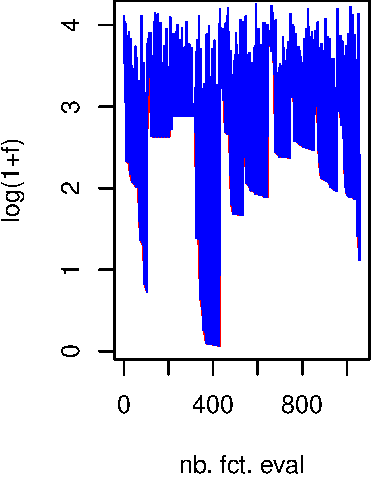
\includegraphics[width=\textwidth]{rastrigin_budget1000_restart10_f-crop.pdf}
\end{minipage}
\vspace{0.7cm}
\begin{minipage}[t]{0.4\textwidth}
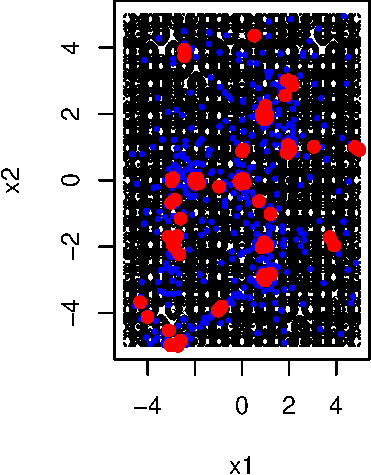
\includegraphics[width=\textwidth]{rastrigin_budget1000_restart10_x-crop.pdf}
\end{minipage}
}
\end{center}

\vskip\baselineskip
\noindent 6. 
Régularisation vs. nombre de données: le plan d'expérience donne les résultats suivants:
\begin{table}[H]
\begin{tabular}{|l|c|c|c|}
\hline
~ & $\lambda=0.01$ &$\lambda=0.1$ &$\lambda=1$\\ 
\hline
\texttt{ntrain=5}& 0.62266703 &0.53166419 &\textcolor{red}{0.5217468}\\
\hline
\texttt{ntrain=10}& 0.66836290& \textcolor{red}{0.21722179}& 0.4202079\\
\hline
\texttt{ntrain=50}& \textcolor{red}{0.05191297}& 0.06292801& 0.4229770\\
\hline
\end{tabular}
\caption{Root Mean Square Error sur ensemble de test, \texttt{ntest=100}.
En rouge: plus faible erreur par ligne (par nombre de données d'apprentissage).}
\end{table}
On remarque que quand il y a peu de données, il est préférable de beaucoup régulariser
($\lambda=1$ est mieux avec 5 points d'apprentissage) et vice versa, avec 
beaucoup de données (50 points) il n'est pas vraiment nécessaire de régulariser.
Intuitivement, cela peut être vu comme un rapport entre la flexibilité du réseau (qui augmente quand 
$\lambda$ décroît) et le nombre de points d'apprentissage qui contraignent le réseau à passer par eux:
un réseau flexible et peu contraint (maintenu) pour prédire n'importe quoi entre les points d'apprentissage, 
il généralise mal.\\
\texttt{rmsetrain} augmente avec $\lambda$ car l'accent est de plus en plus mis sur la minimisation de $\lVert x \rVert_1$. D'ailleurs, quand $\lambda$ est grand, de nombreuses composantes du réseau sont nulles, d'autant plus qu'il y a peu de points de données.

\end{document}
